% Section 3.3: System Architecture Overview

\section{3.3 System Architecture Overview}
\label{sec:architecture-overview}
\addcontentsline{toc}{section}{3.3 System Architecture Overview}

\lettrine{T}{his section} presents Symphony's architectural foundation based on the Harmonic Hexagonal Actor Architecture (H²A²) and the multi-phase bootstrap process. The architecture emphasizes separation of concerns, fault isolation, and intelligent orchestration for AI-first development.

\subsection*{3.3.1 H²A² Architecture and Design Philosophy}
\addcontentsline{toc}{subsection}{3.3.1 H²A² Architecture and Design Philosophy}

Symphony's architecture embraces a microkernel design philosophy prioritizing modularity and extensibility. The foundation rests on the Harmonic Hexagonal Actor Architecture (H²A²), combining hexagonal architecture with actor-based concurrency models.

The H²A² Architecture establishes clear boundaries between domain logic and infrastructure adapters. The Domain Core maintains workflow definitions, extension policies, and orchestration logic, operating independently through well-defined port interfaces. The architecture consists of four key layers:

\textbf{Layer 1a: Domain Core Components}

The Domain Core contains three essential components: OrchestrationEngine for workflow scheduling, WorkflowDefinitions for templates and validation, and ExtensionPolicies for security rules. These define system behavior independent of implementation details.


\begin{figure}[H]
\centering
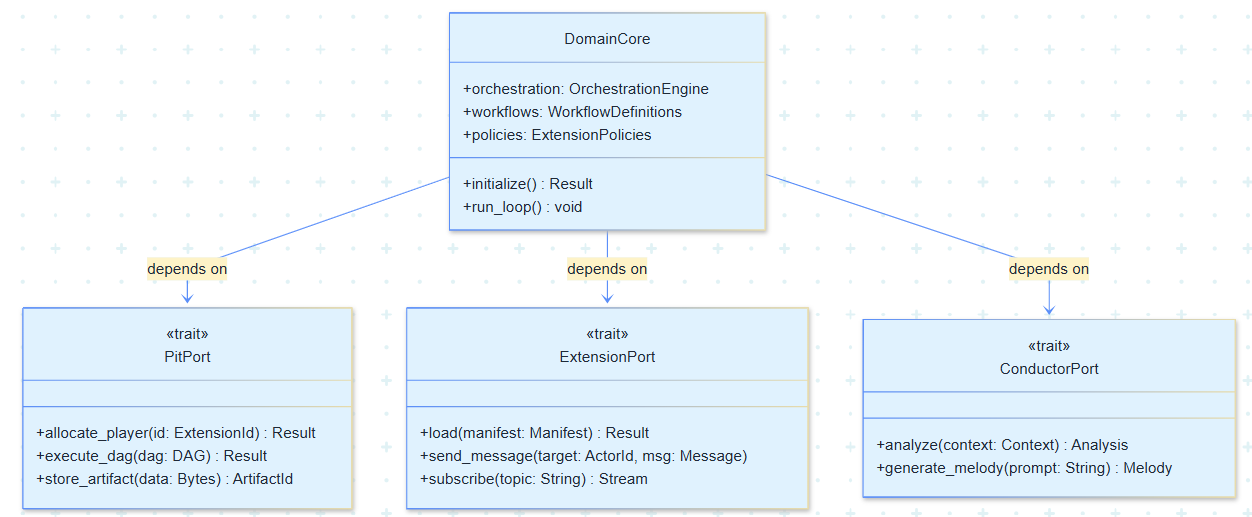
\includegraphics[width=1.15\textwidth]{images/diagrams/class_diagram/seperate_1_h2a2_architecture_domain_adapters/H²A² Architecture Part1 part1.png}
\caption{H²A² Architecture - Domain Core Components}
\label{fig:3.6a-h2a2-domain-components}
\end{figure}

\clearpage
\textbf{Layer 1b: Port Interfaces}

The Domain Core depends on abstract port interfaces that define contracts for external interactions. PitPort handles player allocation, DAG execution, and artifact storage. ExtensionPort manages extension loading, messaging, and topic subscriptions. ConductorPort provides context analysis and melody generation capabilities. TextEditingPort handles text insertion, deletion, and editing operations. These interfaces enable the core to remain independent of concrete implementations as illustrated in Figure 3.3.

\begin{figure}[H]
\centering
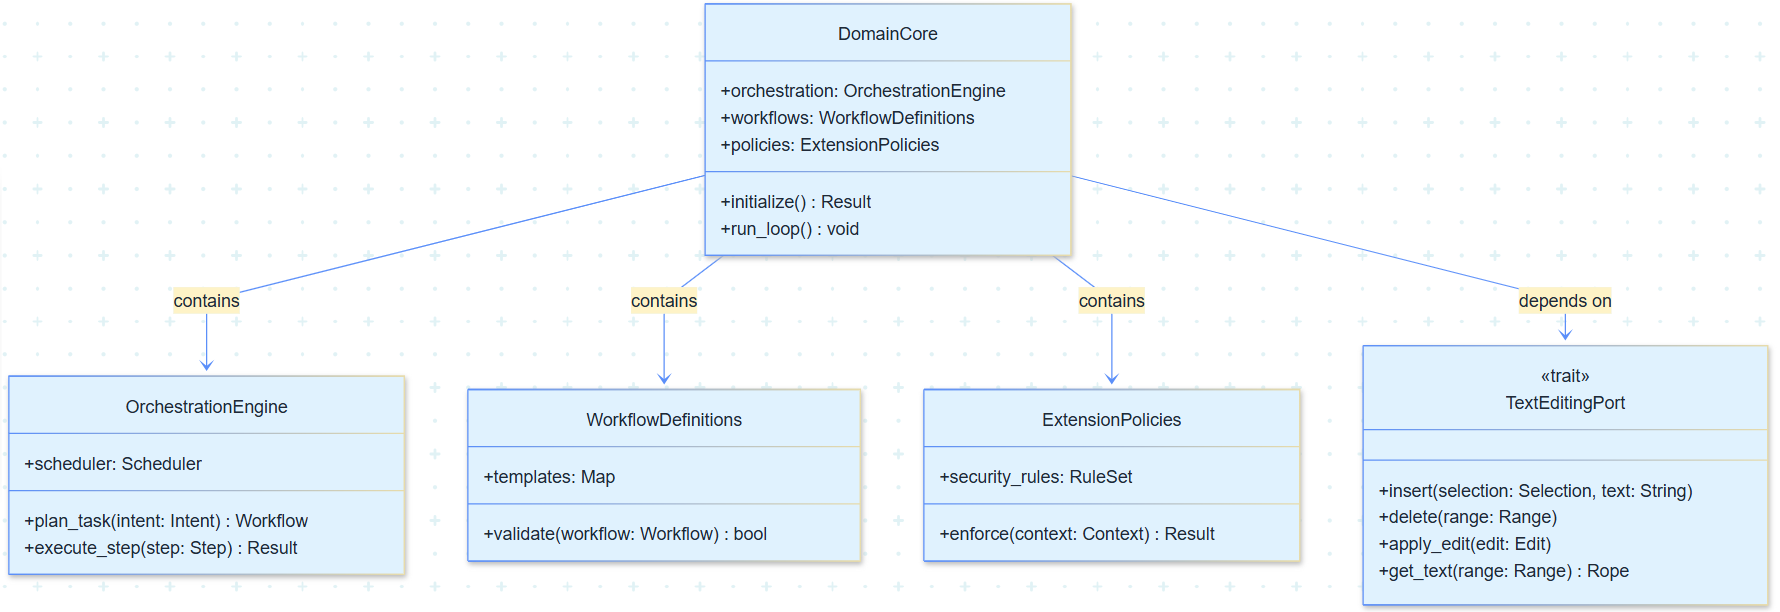
\includegraphics[width=1.15\textwidth]{images/diagrams/class_diagram/seperate_1_h2a2_architecture_domain_adapters/H²A² Architecture Part1 part2.png}
\caption{H²A² Architecture - Port Interfaces Layer}
\label{fig:3.7-h2a2-ports}
\end{figure}

\textbf{Layer 2: Extension and Orchestration Adapters}

The second layer handles extension management and AI orchestration. The ActorExtensionAdapter manages The Grand Stage actor-based extension system, coordinating instruments, operators, and motifs through the actor registry and supervisor strategy. The ConductorAdapter bridges communication with the Python-based reinforcement learning model, enabling intelligent workflow generation through context analysis and melody generation capabilities as illustrated in Figure 3.4.

\begin{figure}[H]
\centering
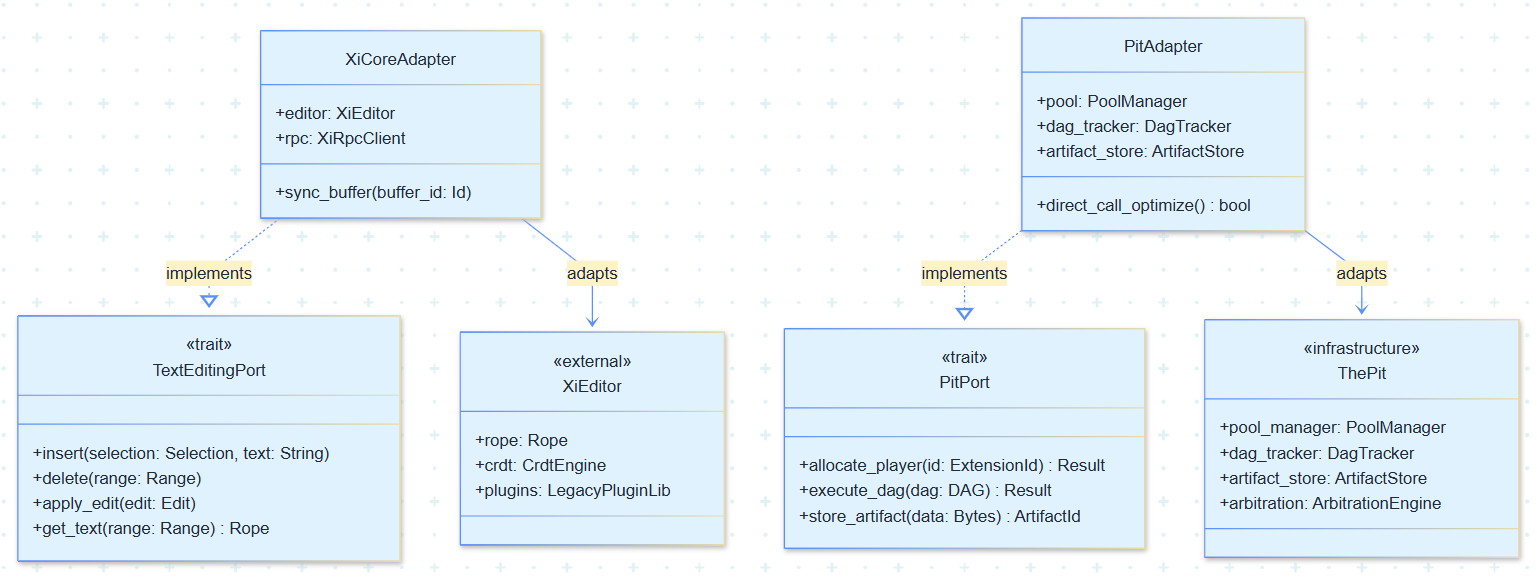
\includegraphics[width=0.95\textwidth]{images/diagrams/class_diagram/seperate_1_h2a2_architecture_domain_adapters/H²A² Architecture Part2.png}
\caption{H²A² Architecture - Extension and Orchestration Adapters Layer}
\label{fig:3.8-h2a2-orchestration}
\end{figure}

\textbf{Layer 3: Domain Core and Port Interfaces}

The third layer represents the Domain Core with its abstract port interfaces. The core contains the OrchestrationEngine, WorkflowDefinitions, and ExtensionPolicies that define system behavior at a conceptual level. Port interfaces (TextEditingPort, PitPort, ExtensionPort, ConductorPort) define contracts for external interactions without specifying implementation details. This separation enables the system to remain adaptable to changing requirements without requiring fundamental redesigns as illustrated in Figure 3.5.

\begin{figure}[H]
\centering
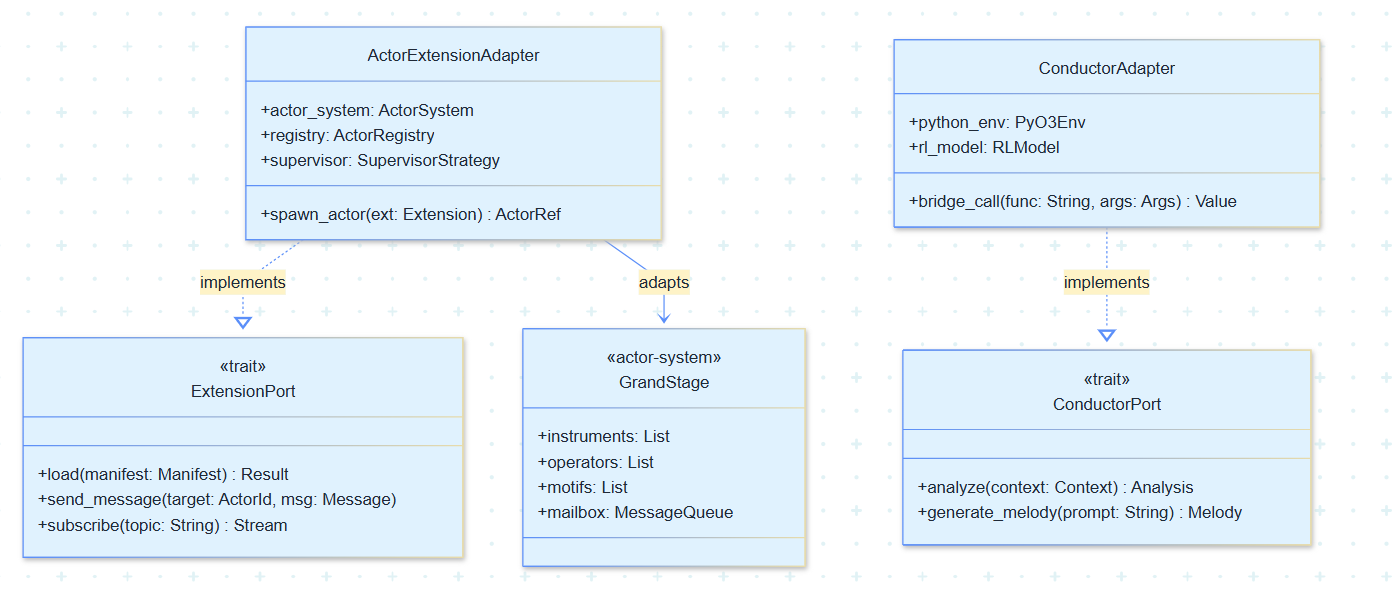
\includegraphics[width=1.15\textwidth]{images/diagrams/class_diagram/seperate_1_h2a2_architecture_domain_adapters/H²A² Architecture Part3.png}
\caption{H²A² Architecture - Domain Core and Port Interfaces Layer}
\label{fig:3.9-h2a2-domain}
\end{figure}

% The microkernel philosophy keeps the core system minimal while delegating specialized functionality to extensions. This contrasts with monolithic IDE architectures that bundle extensive functionality into the core, resulting in bloated applications with slow startup times. Symphony's microkernel contains only essential primitives for orchestration, extension management, and system coordination, while all other capabilities are provided through dynamically loaded extensions.

\clearpage
\subsection*{3.3.2 System Bootstrap and Initialization}
\addcontentsline{toc}{subsection}{3.3.2 System Bootstrap and Initialization}

Symphony's initialization follows a carefully orchestrated bootstrap process through five distinct phases as shown in Figure 3.6, each building upon previous phases with dependency satisfaction and health verification at each stage:

\begin{compactlist}
    \item \textbf{Foundation Phase}: Establishes type system, loads configuration, initializes core orchestration engine
    \item \textbf{IPC Phase}: Sets up inter-process communication infrastructure for extension communication
    \item \textbf{Pit Phase}: Initializes high-performance in-process components (Pool Manager, DAG Tracker, Artifact Store, Arbitration Engine, Stale Manager)
    \item \textbf{Conductor Phase}: Loads Python-based RL model, establishes PyO3 bindings for Rust-Python communication
    \item \textbf{UI Phase}: Brings up user interface, establishes WebSocket connections, performs comprehensive health checks
\end{compactlist}

The architectural design incorporates sophisticated error handling and recovery mechanisms. If any bootstrap phase encounters errors, the system automatically initiates rollback procedures, cleanly shutting down successfully initialized components and returning to a safe state. This rollback capability extends to runtime operations, where component failures are isolated to prevent cascading failures.

The H²A² Architecture's separation of concerns provides significant benefits: new capabilities can be added through additional adapters without modifying the Domain Core, infrastructure components can be upgraded by providing new adapter implementations satisfying existing port interfaces, and comprehensive testing is facilitated through isolated Domain Core testing with mock implementations and adapter testing against port interface contracts.

\begin{figure}[H]
\centering
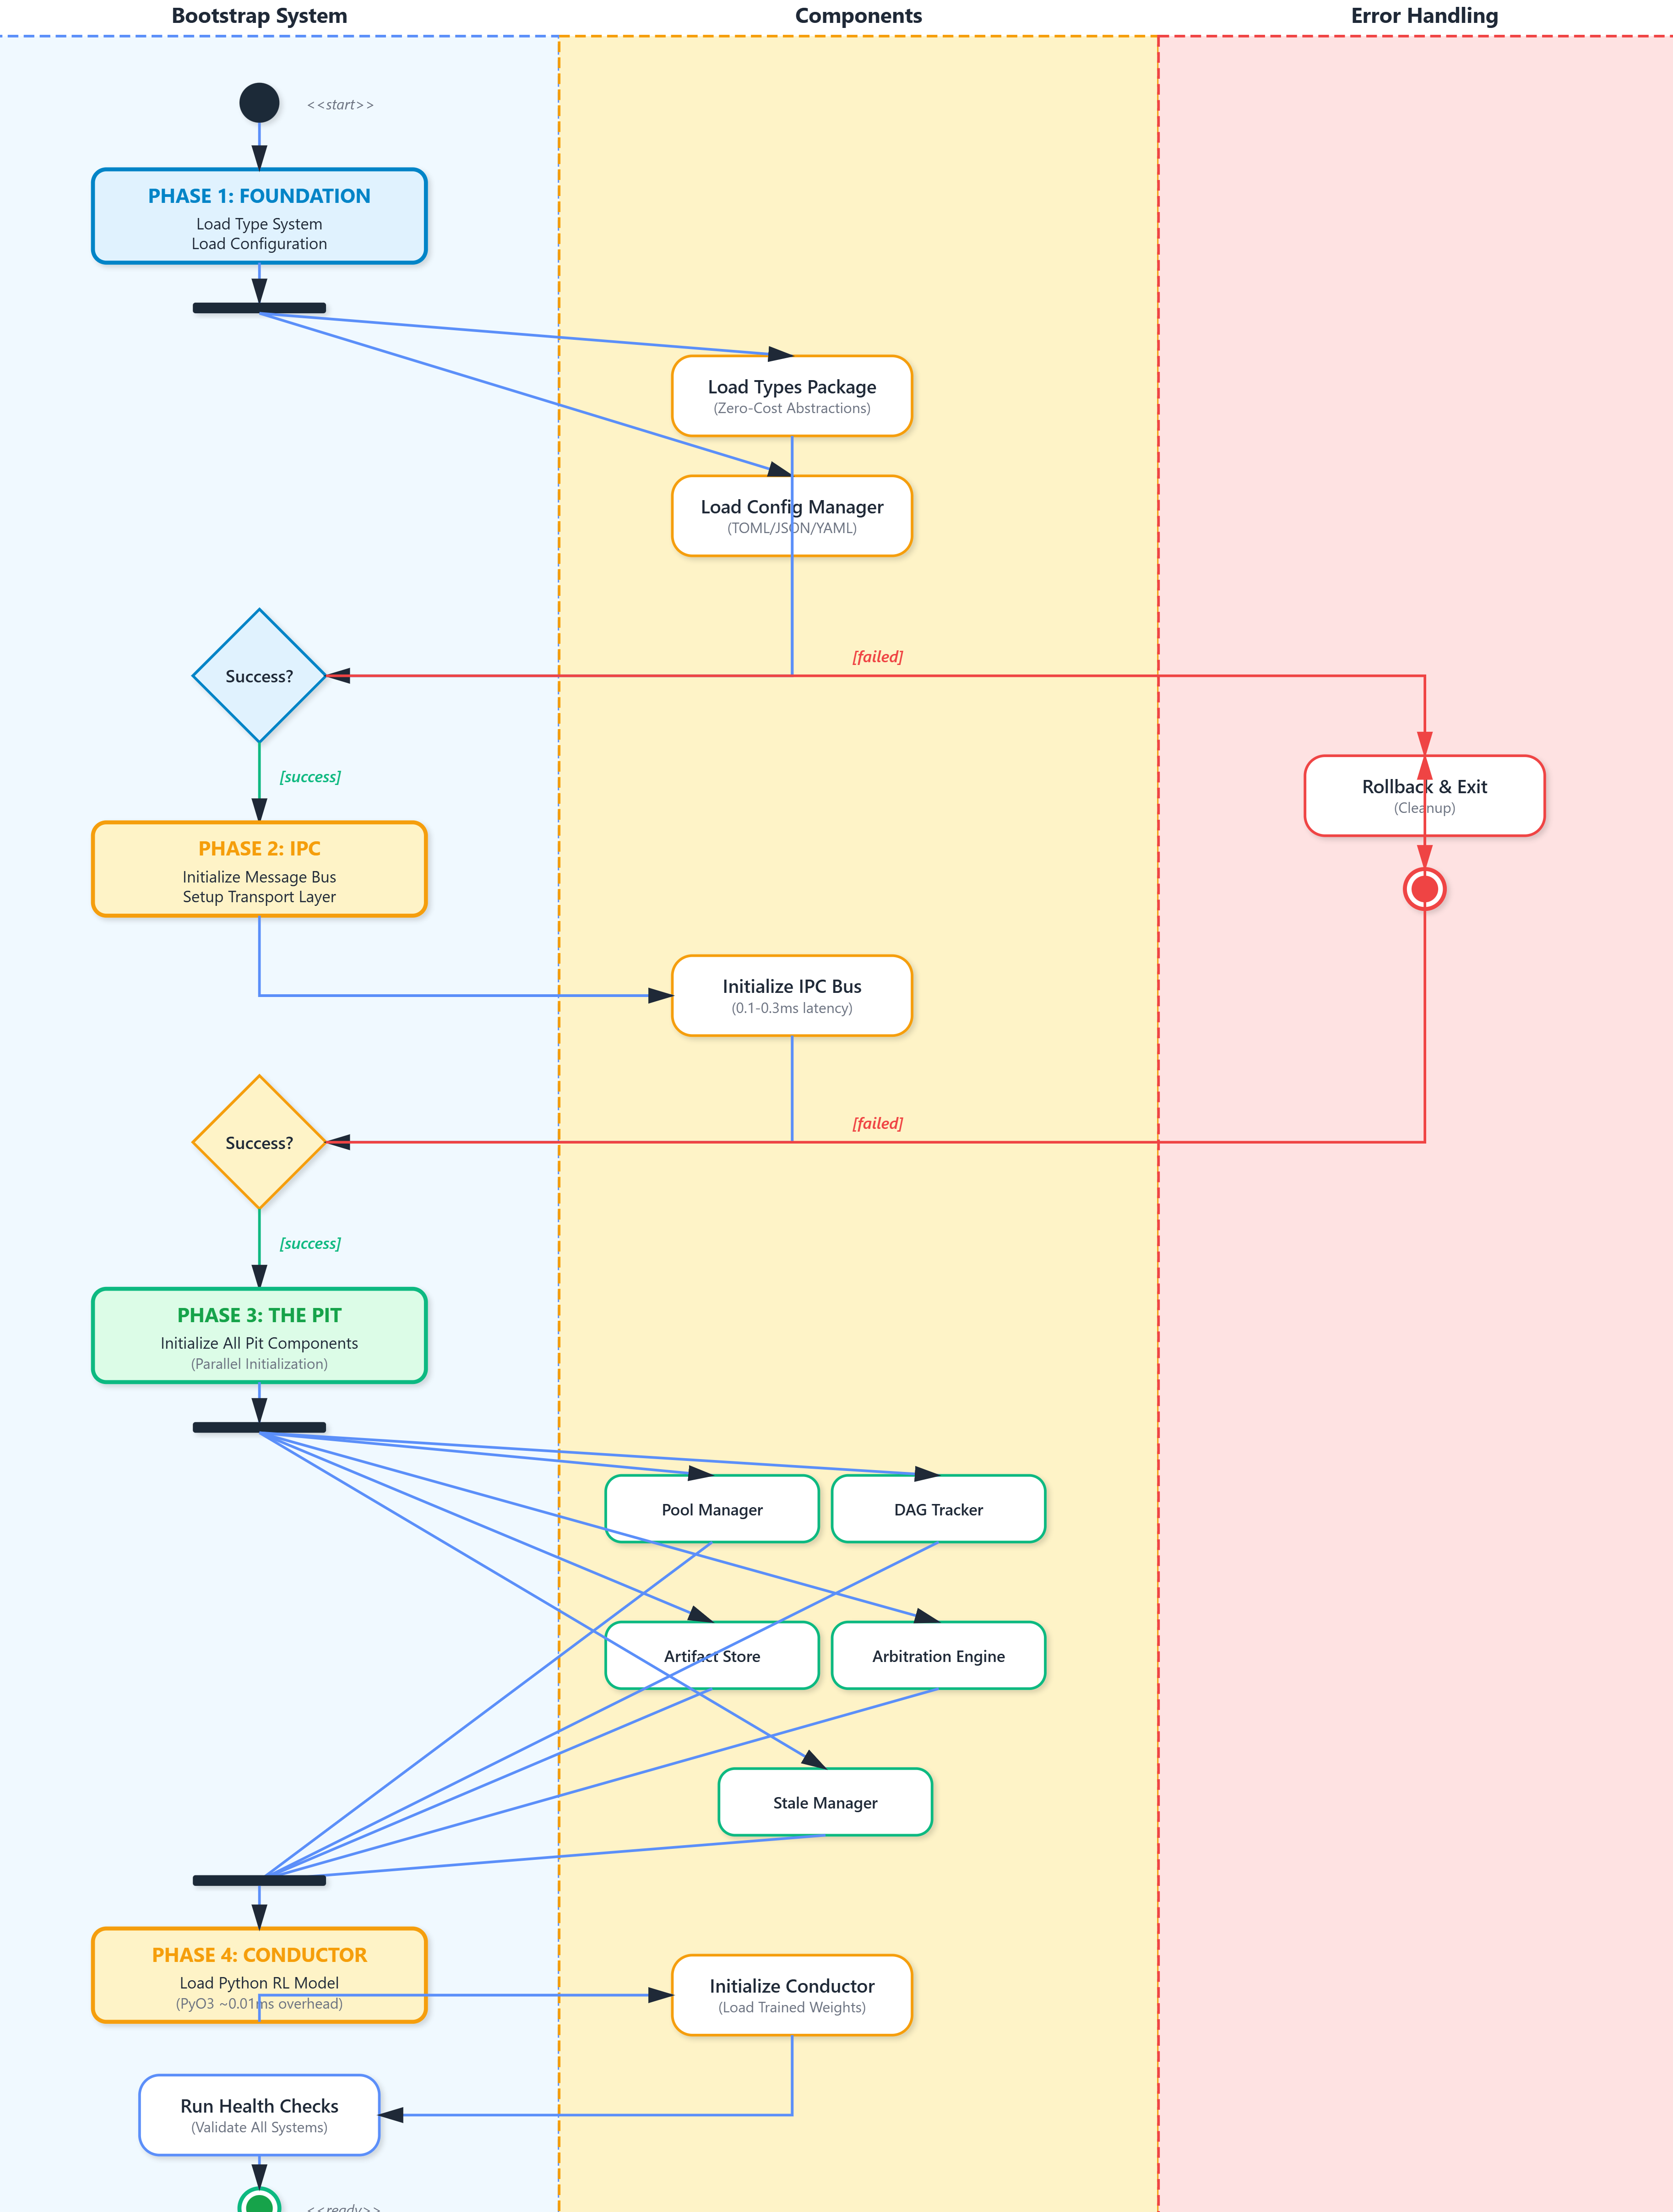
\includegraphics[width=1.25\textwidth]{images/diagrams/activity_diagram/symphony-system-bootstrap.png}
\caption{System Bootstrap Process}
\label{fig:3.10}
\end{figure}


